\subsection{現状の開発成果}
\label{section:current-status}

XRでのマルチアプリケーション・マルチタスクの作業環境を実現するためには,
複数のアプリケーションの描画情報を1つの空間に合成して表示したり,
入力デバイスからの入力を適切なアプリケーションに割り振ったりする,
2D デスクトップ環境でのWindowing Systemの機能が必要となる.
そこで本プロジェクトでは未踏IT人材発掘・育成事業の支援を受けてXR向けのWindowing System,
"ZIGEN"を開発してきた.

ZIGENではWindowing SystemのライブラリであるWaylandの上で,XR用にディスプレイサーバと
アプリケーション間のプロトコルを定義し,参照実装としてのディスプレイサーバ, "ZEN" を実装した.
また既存の2Dアプリケーション(Google Chromeなど)を表示するためのアプリケーションである
"zmonitors"やその他サンプルのアプリケーションを実装した.
これによって主な特徴として以下のことができるようになっている.

\begin{enumerate}
  \item 空間の一部を占めるような複数のアプリケーションをそれぞれ起動し,
        同時に表示する(図\ref{fig:multi-app}).\\
        それぞれのアプリケーションはターミナルなどからプロセスとして立ち上げ,
        % textlint-disable
        OpenGLに似たAPIのZIGENプロトコルに従って頂点バッファ・頂点配列・テクスチャ・
        シェーダ(GLSL)・その他オプションをディスプレイサーバに伝えることで描画を行う.
        % textlint-enable
        ディスプレイサーバ側では受け取った描画情報を各アプリケーションどうしの
        前後関係などが正しく考慮された形で合成し,1つの空間に描画している.
        各アプリケーションはOpenGLで直接描画する場合とほとんど同じインターフェースで
        描画できるため,描画の自由度は大きく損なわない.また他のアプリケーションのことを
        知らずに描画が行え,開発元の違うアプリケーションどうしでも自然に重ね合わされる.
  \item Rayとキーボードを用いて適切に入力をアプリケーションに伝えられる
        (図\ref{fig:ray-input}). \\
        ZIGENではRay(半直線)とキーボードを用いてアプリケーションを操作する.
        Rayは2Dデスクトップのポインタに相当し,アプリケーションへのクリックやスクロール,
        ドラッグといった操作を与える.さらに,Rayによってアプリケーションへ
        フォーカスでき,キーボードイベントはフォーカスしたアプリケーションへのみ渡される.
  \item 既存の2Dアプリケーションを利用できる(図\ref{fig:2d-apps}).
        Google Chromeなどの既存の2Dアプリケーションが修正なしでそのまま動作し,
        Rayを用いて操作できる(Rayと2Dウィンドウとの交点がカーソルとして機能する.).
        この機能を提供するために作成した"zmonitors"というソフトウェアは画面共有のような
        仕組みを用いるのではなく,図\ref{fig:zmonitors}のように2Dのディスプレイサーバとして
        Google Chromeなどと2D Windowing System(Wayland)のプロトコルでやりとりを
        行いつつ,かつ3DアプリケーションとしてZIGENディスプレイサーバとやりとりを行い,
        3D空間上に2Dアプリケーションを表示している.画面共有やVNCなどではなく,
        ディスプレイサーバから実装することによって,画面更新をより効率的に行えたり,
        ヘッドマウンテッドディスプレイ(以降 HMD)と2Dアプリケーションが完全にフレーム同期を
        行えたりする利点がある.これを実現するためにZIGENのプロトコルは既存の
        2D Windowing Systemと変換可能に設計されている.
  \item 2Dと3Dの垣根を越えたドラッグ \& ドロップ(図\ref{fig:dnd}). \\
        ZIGENでは既存の2Dアプリケーションと3Dアプリケーションとの間でドラッグ \& ドロップが
        可能である.このようなことが可能であるのもZIGENが2DのWindowing Systemと
        変換可能に設計され,zmonitorsが2Dディスプレイサーバから実装している利点であり,
        このような2Dと3D アプリケーション間のドラッグ \& ドロップを実装したのは
        調べる限り世界で初である.
\end{enumerate}

開発成果物のクオリティなどに関しては是非"http://..."にアップロードしたデモ動画をご覧
いただきたい. % TODO: Upload デモ


\begin{figure}[htbp]
  \begin{minipage}[t]{0.50\linewidth}
    \centering
    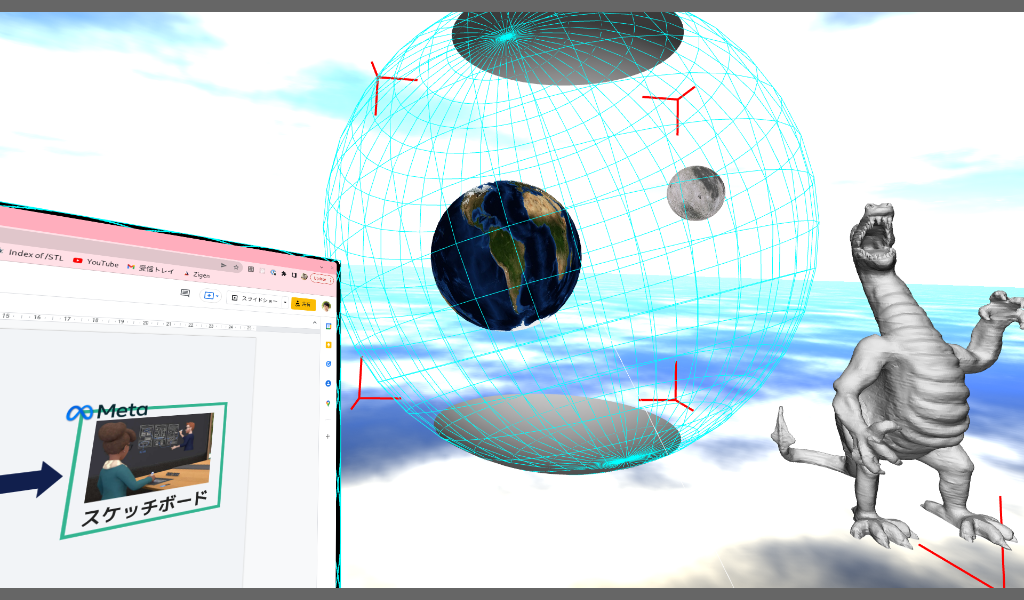
\includegraphics[keepaspectratio, width=\linewidth]{fig/multi-app.png}
    \caption{
      複数3Dアプリケーションの表示.左は既存の2Dアプリケーション(Google Chrome)
      中心はサンプルで作成した天体を表示・編集するアプリケーション,
      右は3Dファイルを表示するアプリケーション.また背景の空も1つのアプリケーションであり,
      ユーザが任意に変更可能である.
    }
    \label{fig:multi-app}
  \end{minipage}
  \begin{minipage}[t]{0.50\linewidth}
    \centering
    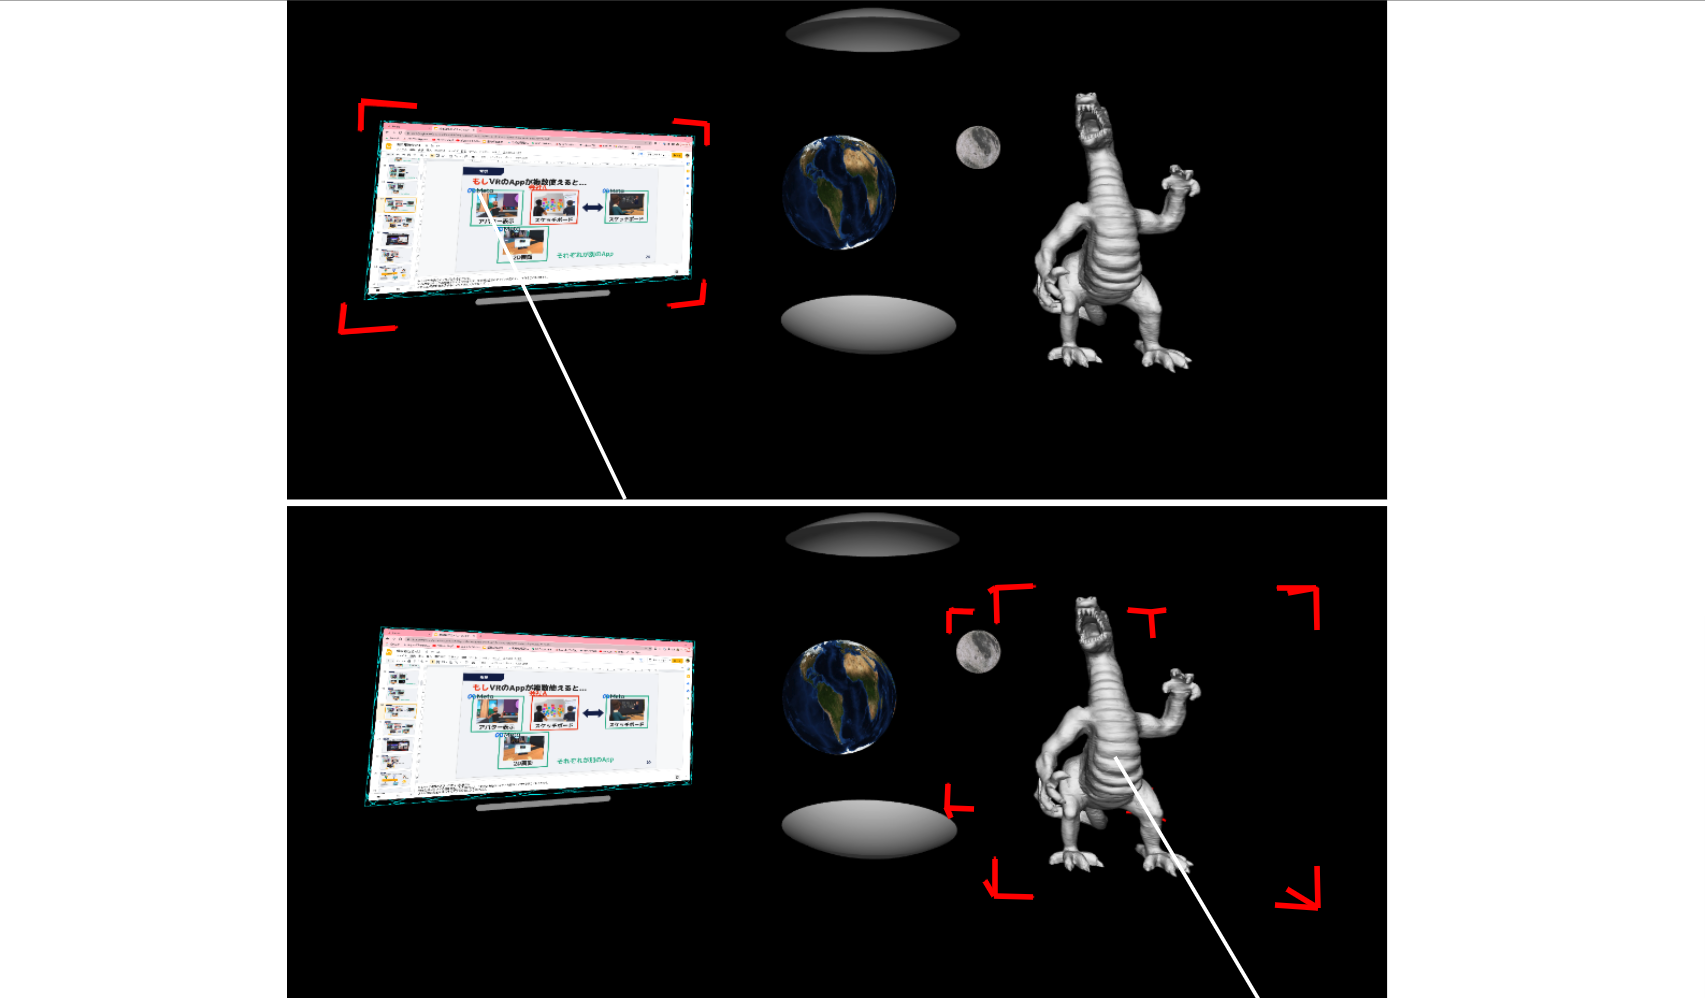
\includegraphics[keepaspectratio, width=\linewidth]{fig/ray-input.png}
    \caption{
      Rayによって3Dアプリケーションへのフォーカスを切り替えている様子.
      上段は一番左のアプリケーションに,下段は真ん中のアプリケーションにフォーカスしており,
      アプリケーションがハイライトされている様子がわかる.
    }
    \label{fig:ray-input}
  \end{minipage}
\end{figure}

\begin{figure}[htbp]
  \begin{minipage}[t]{0.50\linewidth}
    \centering
    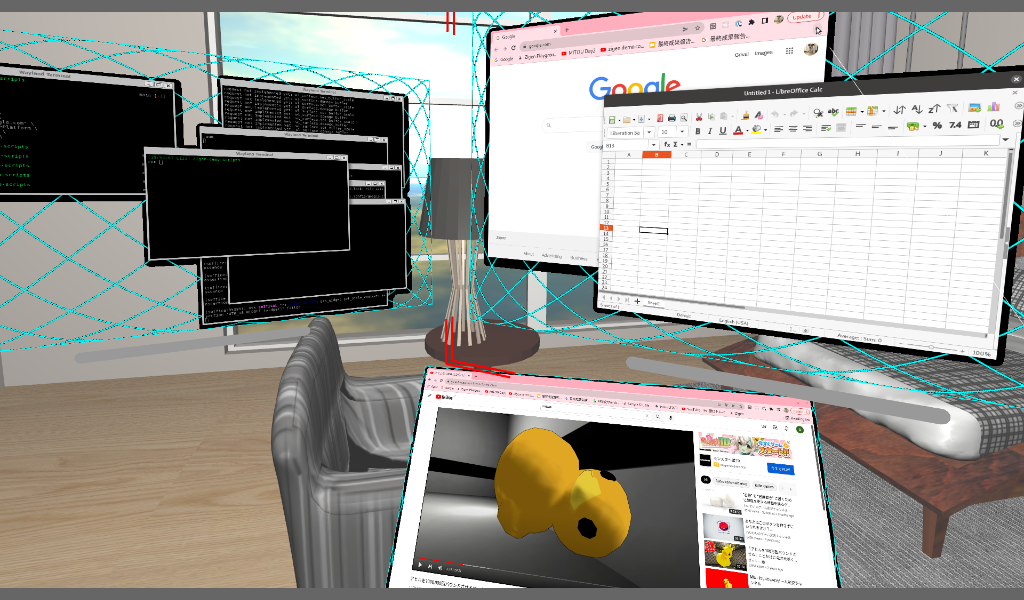
\includegraphics[keepaspectratio, width=\linewidth]{fig/2d-apps.png}
    \caption{
      ブラウザなどの既存の2Dアプリケーションが修正なしでそのまま動作する.
    }
    \label{fig:2d-apps}
  \end{minipage}
  \begin{minipage}[t]{0.50\linewidth}
    \centering
    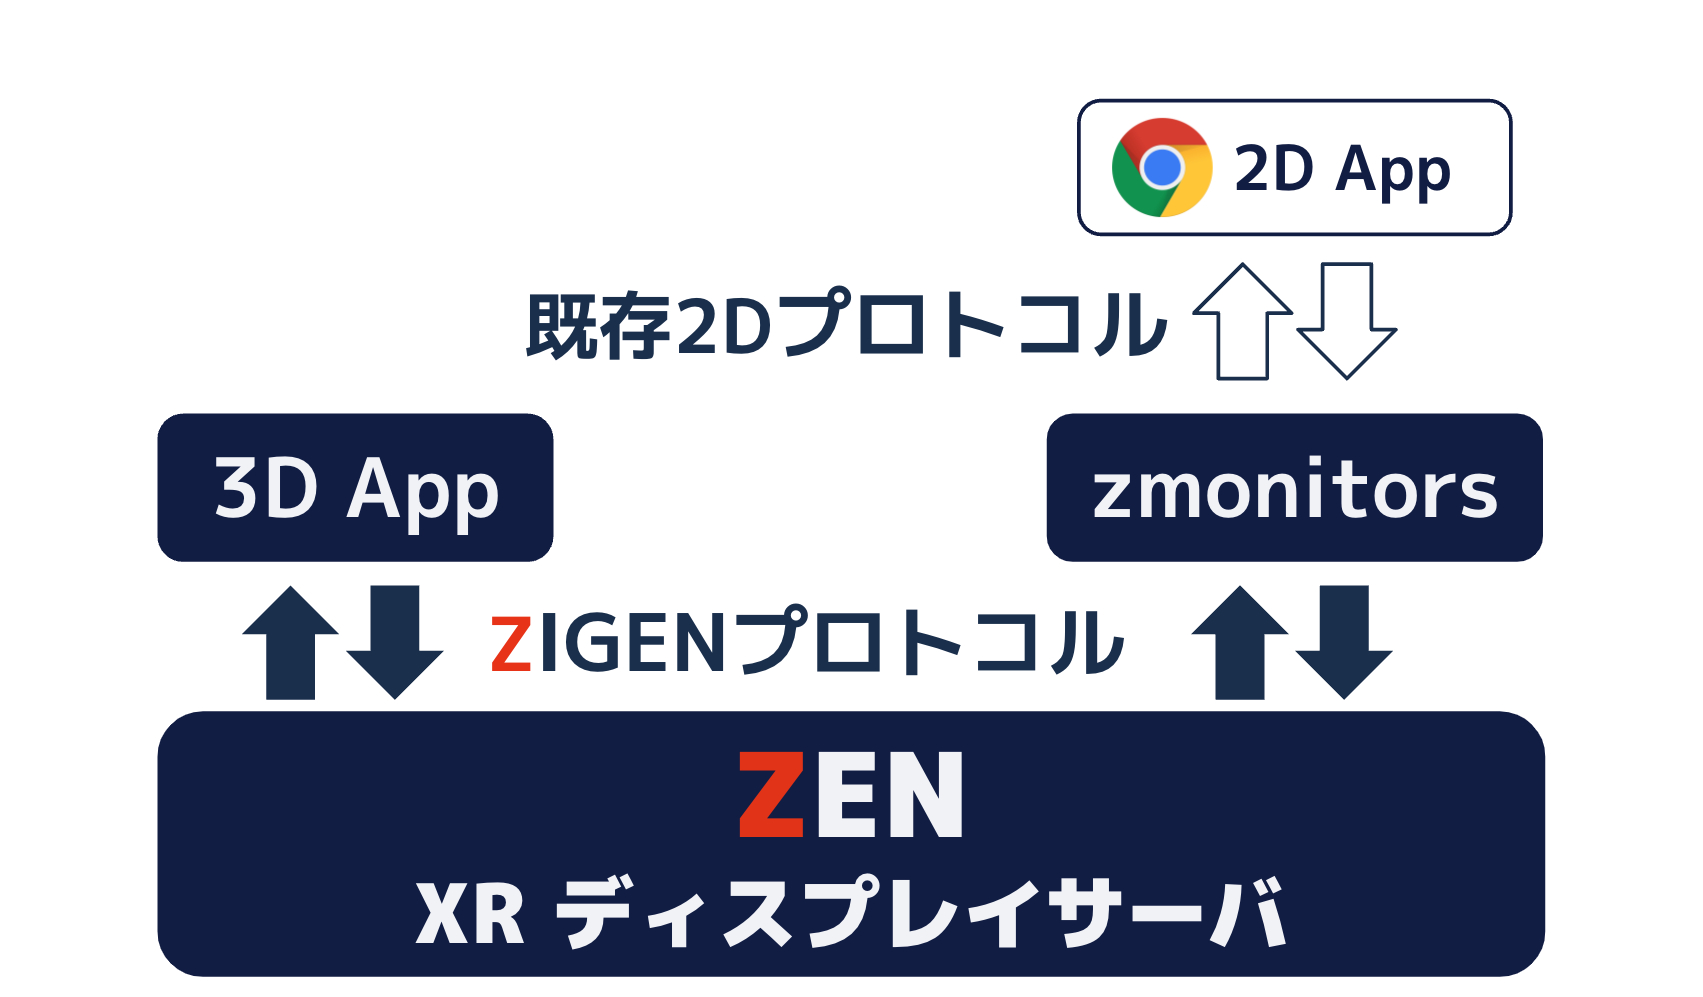
\includegraphics[keepaspectratio, width=\linewidth]{fig/zmonitors.png}
    \caption{
      既存の2Dアプリケーションを3Dアプリケーションに変換するzmonitors.
    }
    \label{fig:zmonitors}
  \end{minipage}
\end{figure}

\begin{figure}[htbp]
  \begin{minipage}[t]{0.50\linewidth}
    \centering
    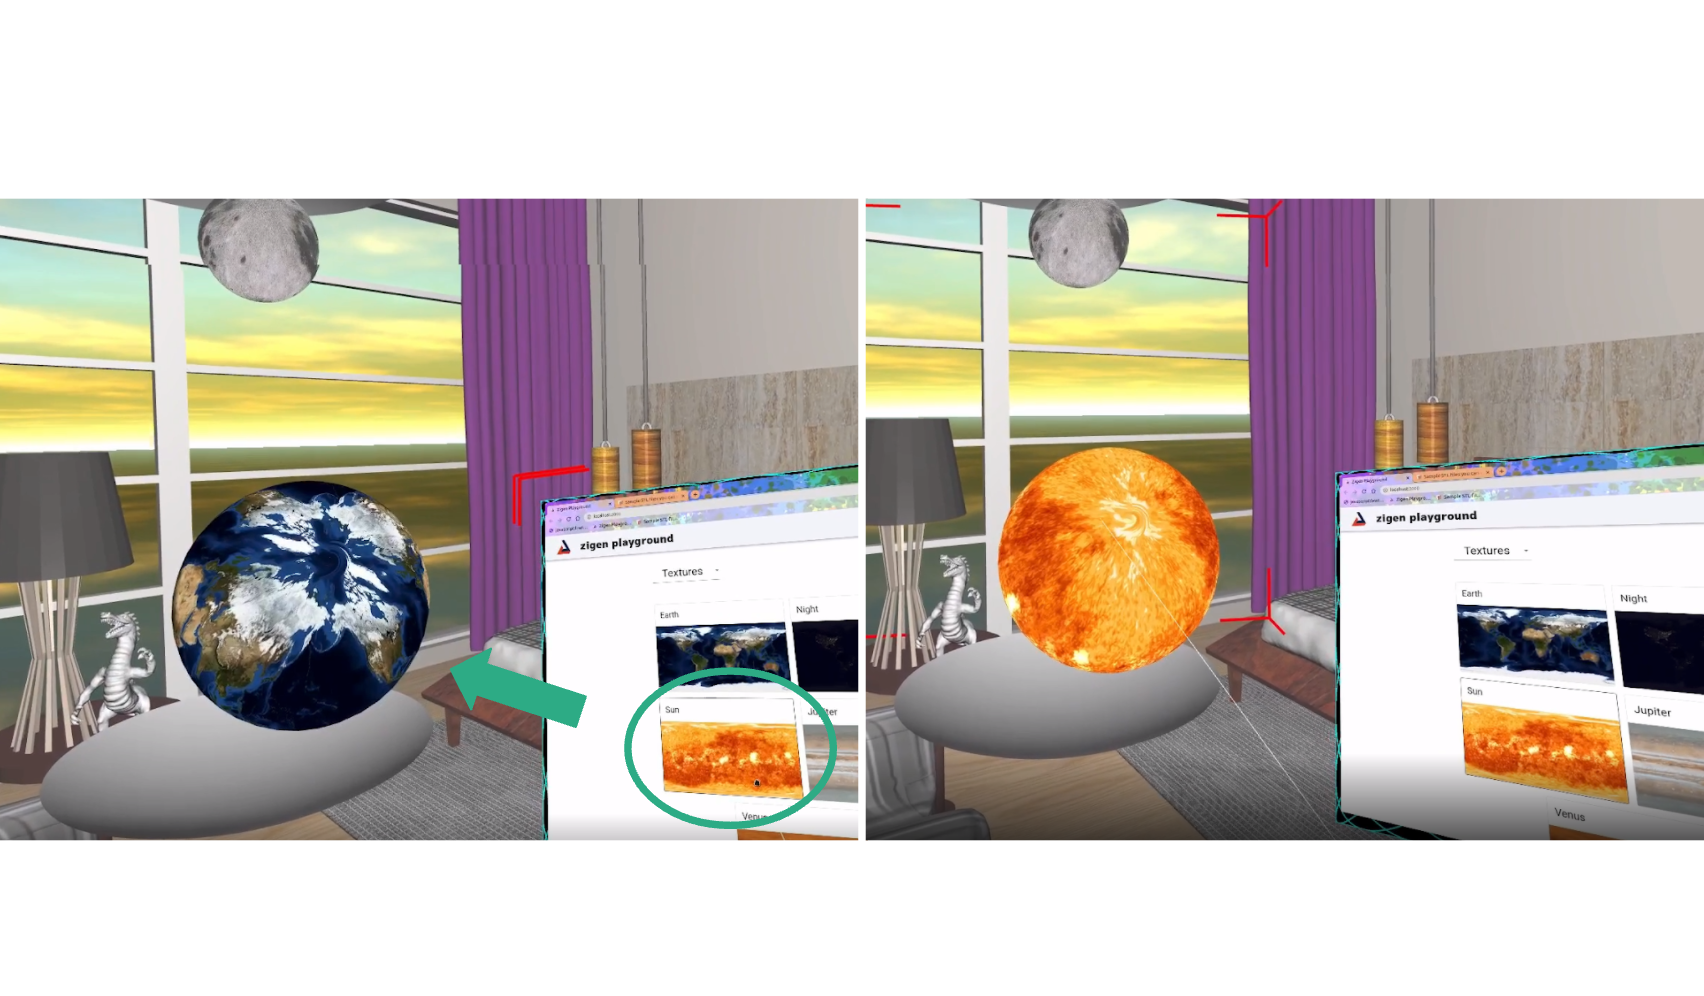
\includegraphics[keepaspectratio, width=\linewidth]{fig/dnd.png}
    \caption{
      Google Chromeから天体を表示・編集する3Dアプリケーションに,天体のテクスチャを
      ドラッグ \& ドロップすることで,天体を地球から太陽に変更する様子.
    }
    \label{fig:dnd}
  \end{minipage}
\end{figure}
